\documentclass[a4paper, 12pt]{article}

\usepackage{graphicx}

\begin{document}

	\title{Optimization of time}
		\author{Nick Wang}
		\date{\today}
	\maketitle	
	
	\pagenumbering{arabic}
	\tableofcontents

	\newpage
	\part{Interpretation of the problem}
		\section{Introduction}
		\paragraph
		\indent In popular video games of the battle royale genre, 100 players are dropped off a plane at the beginning of each round. As I played this game more and more, one question has been asked many many times: How to land on the ground in the shortest time possible? At the time I first asked this question, I was fearful of the mathematics involved in such a problem goes beyond my capability, but with knowledge obtained this year and some basic assumptions, it is possible to approach this problem by dissecting it into smaller components.
		\paragraph
		\indent Another angle this problem can be looked at, with some slight modifications, in a more realistic scenario is when a skydiver wants to parachute to a given location, what is fastest way possible for the skydiver to complete this task?
		\paragraph
		\indent The two approaches to this problem may first seem similar, but they differ slightly. If in a completely realistic environment, meaning a complete replication of what would happen in the real world, the first scenario being a computer simulation would introduce altered physics such as different gravitational acceleration, different air resistance, etc, whereas in the second scenario theses values would reflect the real data. But from a mathematical point of view, the difference in these variables would meant a different coefficient in some equations, while a general equation can be applied onto both scenarios. This work will combine the two approaches for a simple yet accurate representation.
		
		\section{The Problem}
		\paragraph
		\indent The problem told in plain English is as stated: An object, in this case a player, is thrown off an airplane flying in a fixed, predetermined, straight path over a field. The object then proceed to glide in any direction desired while falling downwards towards the ground. Below a certain height is reached, the object then opens up a parachute to slow its descent. The aim is to find the shortest possible time it would take for this object to reach any point on the field.
		\begin{figure}
			\centering
			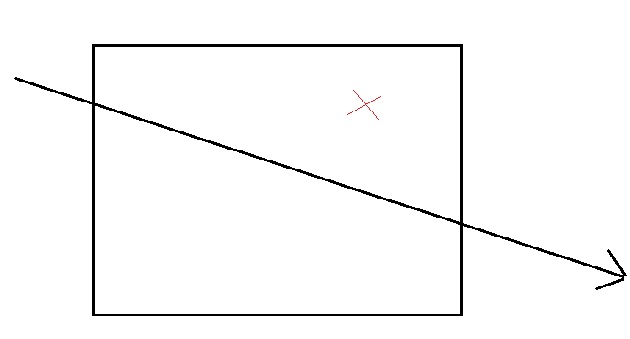
\includegraphics[width=0.8\textwidth]{map.jpg}
			\caption{A simple representation of the scenario. The path is marked by the arrow, and the destination is marked by the "x"}
		\end{figure}

		\section{Mathematical reproduction of the problem}
		\paragraph
		\indent To better understand what is being asked, we need to dissect the problem into its components and understand what are the factors that may affect the time that it would take for an object to reach the ground. The first step is to realize that the total time it will take is the sum of the time this object is on the vehicle following a fixed path at a fixed velocity, stage 1, and the time the object is off the vehicle and is free to control its movement, stage 2. 	
		\begin{figure}[h!]
			\centering
			\begin{minipage}{.5\textwidth}
				\centering
				 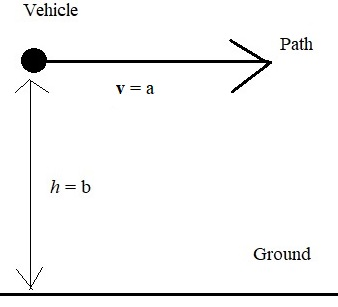
\includegraphics[width=.6\linewidth]{stage1.jpg}
				\caption{Stage1: the object remains on vehicle and travels at velocity v=a at height h = b }
			\end{minipage}%
			\begin{minipage}{.5\textwidth}
			\centering
				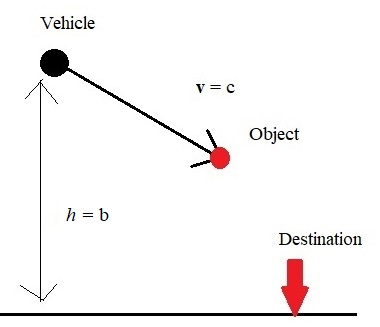
\includegraphics[width=.6\linewidth]{stage2.jpg}
				\caption{Stage2: the object leaves the vehicle at initial height h = b and travels to velocity v =c}
			\end{minipage}
		\end{figure}

		\paragraph	
		\indent During stage 1 since the path and velocity are constant, thus the duration of stage is only dependent on the time at which stage 2 begins, or the arbitrary time the object leaves the vehicle. Thus if stage 2 starts at $t=a$ , then the duration of stage 1 is $a$. Furthermore we can conclude that since velocity is constant, the time required to complete stage1, $t_{stage1}$, is linear.
		\paragraph
		\indent Stage 2 consists of 2 sub-stages, first substage is when the object is first thrown off the vehicle and is in a controlled freefall, where the angle of falling can be manipulated. During this stage the velocity will be taken as a vector quantity, and the three components, or the composite movement in x,y,and z direction will determine overall velocity. The second substage is when the object reach a certain altitude and opens its parachute, which will slow this object to a constant speed, and its velocity will be evaluated similarly to the first substage as a vector. The duration of both stages will mostly be determined by the angle of approach, which changes the horizontal distance traveled throughout the entire stage.
		\paragraph
		\indent Based on these three observations, the following equation of $T_{total}$ at a point $P$ where $t_{stage1}$ and $t_{stage2}$ are known can be deduced: $$T_{total} = t_{stage1} + t_{stage2}$$ Thus $T_{total}$ at another point can also be deduced in relation to point $P$: $$T_{total2} = t_{stage1} + dt_{stage1} + t_{stage2}+dt_{stage2}$$ That $T_{total2}$ is the sum of $T_{total}$ at point $P$ and the difference in duration of $t_{stage1}$ and the difference in duration of $t_{stage2}$. And the desire is that $T_{total2} < T_{total}$, thus: $$T_{total2} - T_{total} \leq 0$$
		$$ t_{stage1} + dt_{stage1} + t_{stage2}+dt_{stage2} - t_{stage1} - t_{stage2} \leq 0$$
		$$ dt_{stage1} + dt_{stage2} \leq 0$$
		This inequality will be further examined in later discussions.

		\section{Assumptions and definitions}
		\paragraph
		\indent The combination of the two stages produce a simplified mathematical representation of the problem. But with further thought we would realize that this representation avoided consideration of factors such as air resistance and terminal velocity. Such factors, as mentioned in the introduction, need to be considered differently in the two different scenarios presented.
		\paragraph
		\indent In the scenario of a computer simulated environment, such values are completely arbitrary to the designer's will. Since this work will not be specific to a single instance of such computer games, some general observations will be made. Thus in this calculation we will redefine the following for the purpose of simplification, and to best reconcile the video game physics and real world physics:
		\begin{enumerate}
			\item[-] Air resistance: Air resistance will be ignored.
			\item[-] Initiation: At the instant the object leaves the vehicle, the object assumes 0 velocity and is stationary relative to the ground.
			\item[-] Terminal velocity: The falling object will reach an arbitrarily defined terminal velocity, and keep falling at this velocity in stage 1 until stage 2 is reached.
			\item[-] Deceleration: The instance stage 2 is reached, the object will release a parachute, and will slow down and descend at terminal velocity, while horizontal velocity will not affect on terminal velocity.
			\item[-] Velocity:The object will travel in any direction at a constant velocity.
		\end{enumerate}
		\paragraph
		\indent The definition of Terminal Velocity needs to be further examined. Terminal Velocity is the velocity at which an object will reach in an atmosphere, where the air resistance is equal to the gravitational acceleration. Terminal Velocity will be reached quickly after an object begins its freefall, or in a different word, the time it takes for the object to reach Terminal Velocity is finite, and as the height of fall increases, this time do not increase, and remain a constant $c$. Thus this time compared to the total time of the fall, as the height of fall changes and approaches infinity, is $$\lim_{x\to\infty} \frac{c}{x} = 0$$ Thus we will assume the time it would take for the object to reach Terminal Velocity is 0.
		\paragraph
		\indent Similarly to Terminal Velocity, the final stages of the fall, after the parachute is released, the player experiences a limited period of deceleration. This period of time, again, is independent of the height of the fall, and is completely arbitrary. In reality one skydiver can release its parachute 3000ft off the ground, another can release it 2000ft off the ground. In the context of this problem, we ignore this period of time and assumes the object can instantly decelerate.
		\paragraph
		\indent Another concept that has to be examined is the velocity of the vehicle in relation to the velocity of the object. It is commonsensical to see that it is unrealistic that the object would travel at a greater velocity than the vehicle, or in reality if a skydiver can fly faster than a plane. Thus in this problem the, strictly speaking, horizontal velocity is always significantly less than that of the vehicle.
		\paragraph
		\indent By setting up the two scenarios of the same problem in this fashion we have greatly simplify the problem into its essence. Nuances like ignoring air resistance will definitely introduce a greater error to the overall calculation, but we hope it is negligible compared to other more important factors.

	\part{Speculations}
		\section{Speculations}
		\paragraph
		\indent With the problem and variables defined, we will now look at the problem as a whole and provide some speculations. As explained in Part I Mathematical Reproduction of the Problem, the overall time is the duration of stage 1 and 2 combined, and the aim is to minimize this sum. Of these two stages it is easy to see that stage 2 is symmetrical to the normal line to the path of the vehicle that passes through the destination point as shown in figure 4.
		\begin{figure}[h]
			\centering
			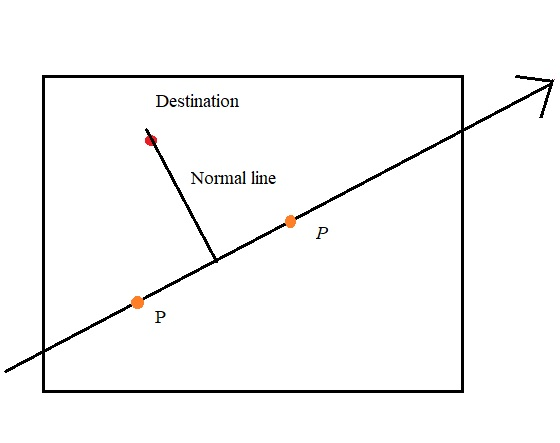
\includegraphics[width=0.8\textwidth]{Symmetry.jpg}
			\caption{As shown above, point P and point $P$ are symmetrical to the normal line}
		\end{figure}
		\paragraph
		\indent Thus the duration of stage2 at any point after the vehicle crosses the normal line has an identical, symmetrical point before the vehicle passes through the normal line. Furthermore the duration of stage1 at any point after the normal line is greater than that before crossing the normal line, as we've concluded in Part I that the duration of stage1 is linear, and the longer the object remains on the vehicle, the longer stage1 is. Thus it is safe to conclude that the smallest $T_{total}$ can only be achieved before crossing the normal line, and $t_{stage1}$ is bounded: $$0 \geq t_{stage1} \geq t_{crossing}$$
		\paragraph
		\indent A further speculation can be made that the furthest distance the object can reach is a radius around the point where the object leaves the vehicle as shown in figure 6, and this radius is limited. Thus if the object leaves the vehicle way too early, or from a mathematical perspective, as the beginning time of stage 2 shifts further towards negative infinity, the object will never reach the desired location. Thus we can conclude that one mustn't leave the vehicle too early.
		\begin{figure}[h!]
			\centering
			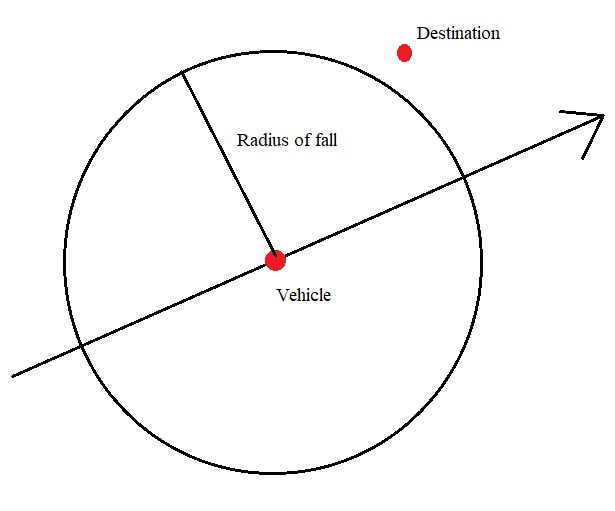
\includegraphics[width=0.8\textwidth]{Radius.jpg}
			\caption{As shown above, the object cannot reach the destination that is outside the maximum radius}
		\end{figure}
		Thus it can be further deduced that the duration of stage1 is $$t_{maxRadius} \geq t_{stage1} \geq t_{crossing}$$

	\part{Calculations}
		\paragraph
		\indent To solve this problem, we need to look back at the inequality we derived in Part I: $$ dt_{stage1} + dt_{stage2} \leq 0$$
		Since the duration of stage1 is linear as discussed above, thus the change in duration of stage1 is a constant:$$\frac{d}{dT_{total}}t_{stage1} = 1 $$
		Thus the inequality can be rewritten as: $$1 + dt_{stage2} \leq 0$$
		$$1 \leq -dt_{stage2}$$
		$$dt_{stage2} \leq -1$$
		\paragraph
		\indent To elaborate on this new inequality, as the vehicle moves along the path, the duration of stage 2 is decreasing. But there will be a point where they amount of duration that would be decreases if the object remained on the vehicle is less than the increase of duration of stage1 by remaining on the vehicle. Thus by finding this point where $dt_{stage2} > -1$, we find the optimal position to leave the vehicle.
		\begin{figure}[h!]
			\centering
			 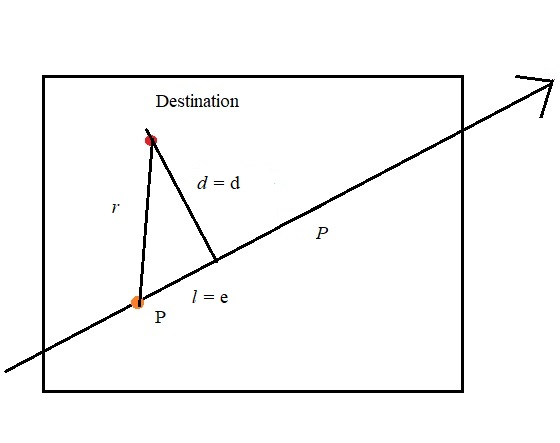
\includegraphics[width=.6\linewidth]{distance.jpg}
			\caption{The horizontal distance, r, the object has to travel }
			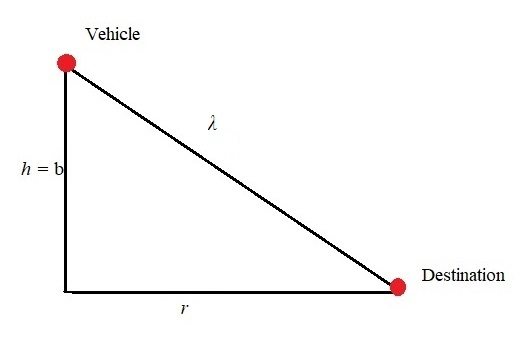
\includegraphics[width=.6\linewidth]{duration.jpg}
			\caption{The total distance, k, the object has to travel }
		\end{figure}
		\paragraph
		\indent To calculate the total distance as shown in figure 6, $d$ would be given since it can be measured as the distance between the destination and the path. We also need to know what the value of $l$ is, and as we've established, the point P is where stage1 ends, and stage1 is bounded in $t_{maxRadius} \geq t_{stage1} \geq t_{crossing}$. Thus we can define t as time before reaching the normal line, and $l = t*v$, where $v$ is the velocity of the vehicle, and: $$r=\sqrt{(tv)^2+d^2}$$
		Referring to figure 7, we can see that $k$ is dependent upon $h$, which is a constant that would be known is a specific example, and $r$, which was just calculated. Thus $$k = \sqrt{b^2+r^2}$$
		Plugging in $r$: $$k = \sqrt{b^2+\sqrt{(tv)^2 + d^2}^2}$$
		Simplifying: $$k = \sqrt{b^2 + (tv)^2 + d^2}$$
		Because $b,v,d$ are all constants, we can take them out and replace them with another constant, where $\alpha = v^2$, $\beta = b^2 + d^2$: $$k = \sqrt{\alpha t^2 + \beta}$$
		Referring to assumptions made in Part I, we assume the object falls at a constant velocity despite the angle, thus $t_{stage2} = \frac{k}{v_{terminal}}$, and $v_{terminal}$ is arbitrarily defined.
		Plugging in $k$: $$ \frac{ \sqrt{\alpha t^2 + \beta}}{v_{terminal}}$$
		Simplifying: $$k = \gamma \sqrt{\alpha t^2 + \beta}, where \gamma = \frac{1}{v_{terminal}}$$
		Taking derivative of $k$: $$k' = 2 \alpha t{( \alpha t^2 + \beta )}^{-1/2}$$
		Thus plugging back into the inequality: $$2 \alpha t {( \alpha t^2 + \beta )}^{-1/2} = -1$$
		Thus solving for $t$ will produce the optimal time.
	\part{Conclusion}
		\section{Conclusion}
		\paragraph
		\indent Upon inspection after completion of the calculations, flaws with this problem can be seen. One assumption in particular about the velocity at which the object falls is especially flawed. It assumes the the object falls at constant velocity at any given angle, which is accurate when the object travels at a very sharp angle to the ground, but if the angle of travel is beyond a certain point, it will behave drastically differently from what is assumed. Additional assumptions would have introduced even greater error to this already flawed solution. With hindsight a better approach to this problem is with computer simulations combined with a better, more robust mathematical model that account for other variables that were not accounted, which would most certainly be significantly more difficult execute. But apart from the inherent complexity of this problem itself, the result concluded from this investigation should very well represent what is described, and achieve what is explicitly desired by the assumptions in this report.

\end{document}

